\begin{homeworkProblem}

\textbf{Three-dimensional Joint Distribution:} Implement a Gibbs sampler to generate samples from the three-dimensional joint distribution shown in the lecture.

\solution

Random variables $X,P,N$ have joint density
$$\pi(x,p,n)\propto \binom{n}{x}p^x(1-p)^{n-1}\dfrac{4^n}{n!}$$
for $x=0,1,2,\ldots,n$, $0<p<1$, and $n=0,1,2,\ldots$. The $p$ variable is continuous, $x$ and $n$ are discrete. We can get the conditional PDF and PMF for the corresponding variables as follows:
\begin{align*}
P_{X|N,P}(X=x|N=n,P=p) &\propto \binom{n}{x}p^x(1-p)^{n-x}\sim \Bin(n,p) \\
f_{P|X,N}(p|X=x,N=n) &\propto p^x(1-p)^{n-x} \sim \Beta(x+1,n-x+1) \\
P_{N|X,P}(N=n|X=x,P=p) &\propto \binom{n}{x}p^x(1-p)^{n-x} = x + Z
\end{align*}
We can get that the last PMF is a shifted Poisson, where $Z\sim\Pois(4(1-p))$. \\
Initially, we set $(x_0,p_0,n_0)\gets(1,0.5,2)$, and we can use Gibbs sampling to generate the samples. \\
The simulated results are as follows:

\begin{figure}[h]
    \centering
    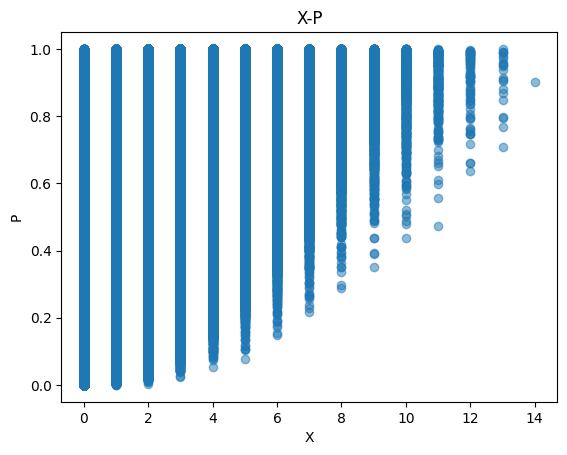
\includegraphics[width=0.4\textwidth]{./figure/p9/X_P.png}
    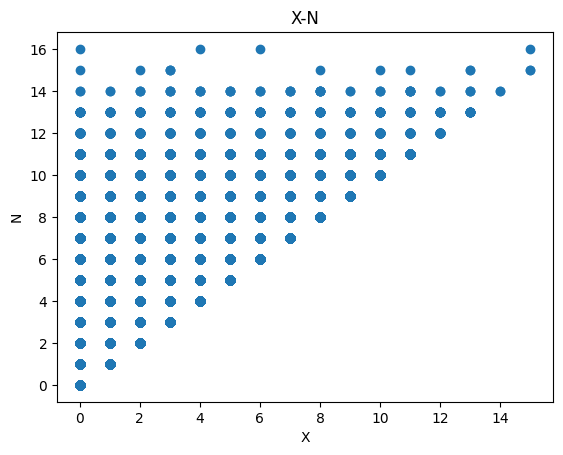
\includegraphics[width=0.4\textwidth]{./figure/p9/X_N.png}
\end{figure}
\begin{figure}[h]
    \centering
    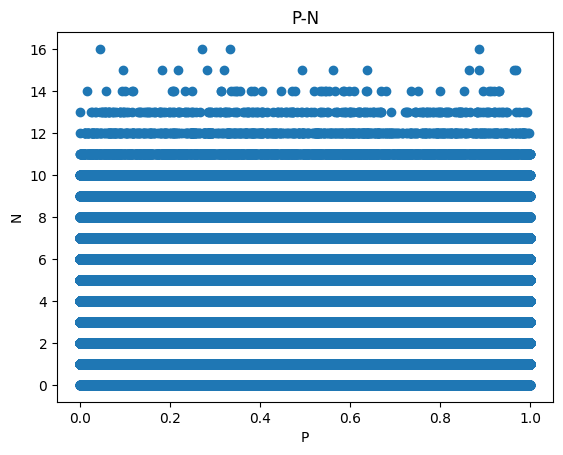
\includegraphics[width=0.49\textwidth]{./figure/p9/P_N.png}
    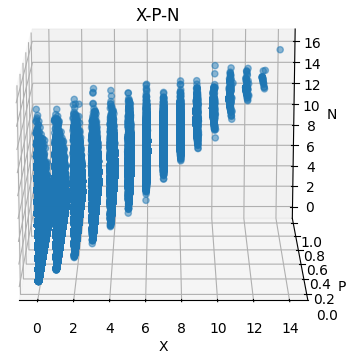
\includegraphics[width=0.4\textwidth]{./figure/p9/X_P_N.png}
\end{figure}

\vspace{1cm}
The estimated marginal distribution are as follows:
\begin{figure}[h]
    \centering
    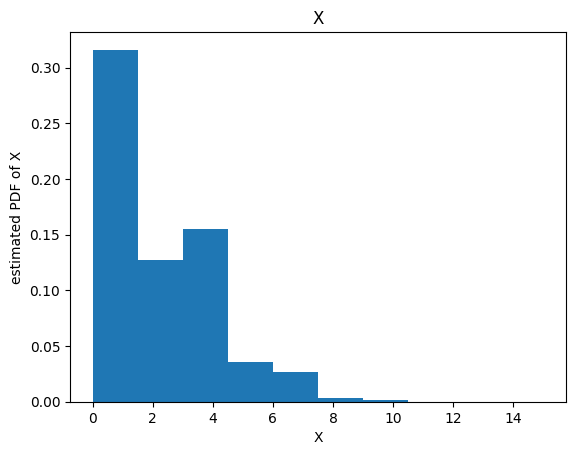
\includegraphics[width=0.4\textwidth]{./figure/p9/X.png}
\end{figure}
\begin{figure}[h]
    \centering
    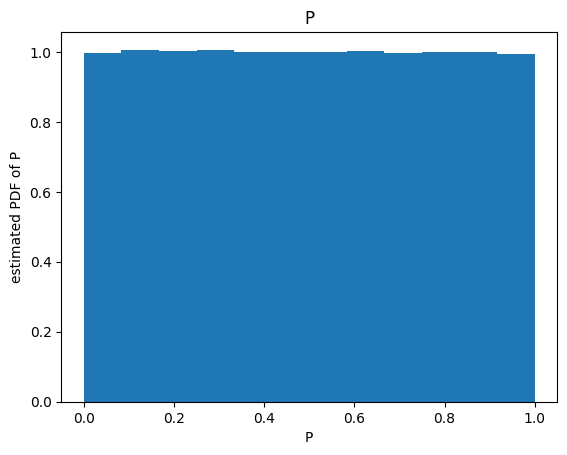
\includegraphics[width=0.4\textwidth]{./figure/p9/P.png}
\end{figure}
\begin{figure}[h]
    \centering
    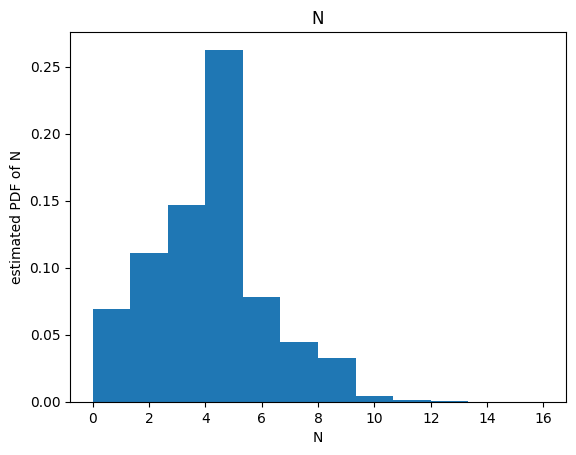
\includegraphics[width=0.4\textwidth]{./figure/p9/N.png}
\end{figure}

\end{homeworkProblem}

\newpage